\documentclass[12pt]{article}
\usepackage[margin=1in]{geometry}
\usepackage{graphicx}
\usepackage{float}
\usepackage{amsmath}
\usepackage{booktabs}
\usepackage{hyperref}
\usepackage{caption}
\usepackage{subcaption}
\usepackage{enumitem}
\usepackage{pifont}

\title{Data Analysis}
\author{Team 2}
\date{\today}

\begin{document}

\maketitle

\section{Introduction}
This section presents an in-depth analysis of the cleaned data set. We observe key variables such as enrollment type, tuition payment behavior, gender, and age range, and aim to identify influential factors that contribute to student academic risk and enrollment decisions. These insights are essential to support data-driven decisions in student retention strategies and institutional planning.


\section{Enrollment Trends}
We analyze enrollment trends based on different factors such as gender, major, and study mode.

\subsection{Gender}
\begin{itemize}
    \item Program 24\\
    - Very popular with both genders.\\
    - Slightly more females (Gender 2) enrolled than males (Gender 1).

    \item Program 16, 27, 52\\
    - Good number of enrollments in both males (Gender 1) and females (Gender 2).

    \item Program 78, 4\\
    - Noticeably more females (Gender 2) enrolled than males (Gender 1).

    \item Program 54, 40, 33, 43\\
    - Strong enrollment of males (Gender 1) but very low enrollment of females (Gender 2).
\end{itemize}

\begin{figure}[H]
    \centering
    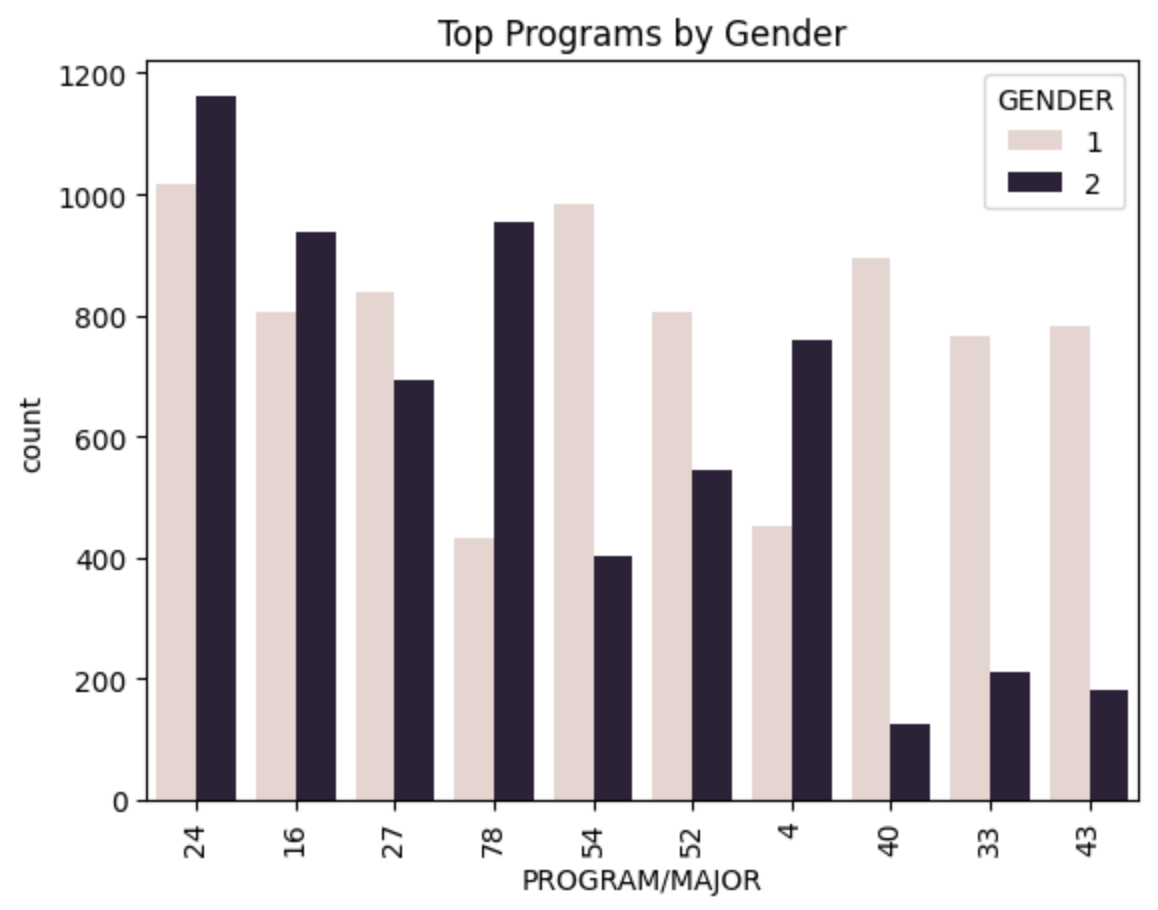
\includegraphics[width=0.7\linewidth]{top_programs_gender.png}
    \caption{Top Programs vs Gender}
\end{figure}

\subsection{Age Range}
\begin{itemize}
    \item Note:\\
    0 : $\leq$ 18\\
    1 : 19-20\\
    2 : 21-23\\
    3 : 24-29\\
    4 : $\leq$ 30
    
    \item Program 24\\
    - Attracts students from all age ranges.\\
    - Particularly popular among students aged $\leq$ 30.

    \item Program 16\\
    - Popularity keeps decreasing with age.

    \item Program 27, 54\\
    - Attracts students aged 24-29 and especially $\geq$ 30.\\
    - Not at all popular among younger students.

    \item Program 4, 40, 43\\
    - Not at all popular among older students aged $\geq$ 30.
    
    \item Program 78, 52, 33\\
    - Fairly popular among students aged upto 24.
\end{itemize}

\begin{figure}[H]
    \centering
    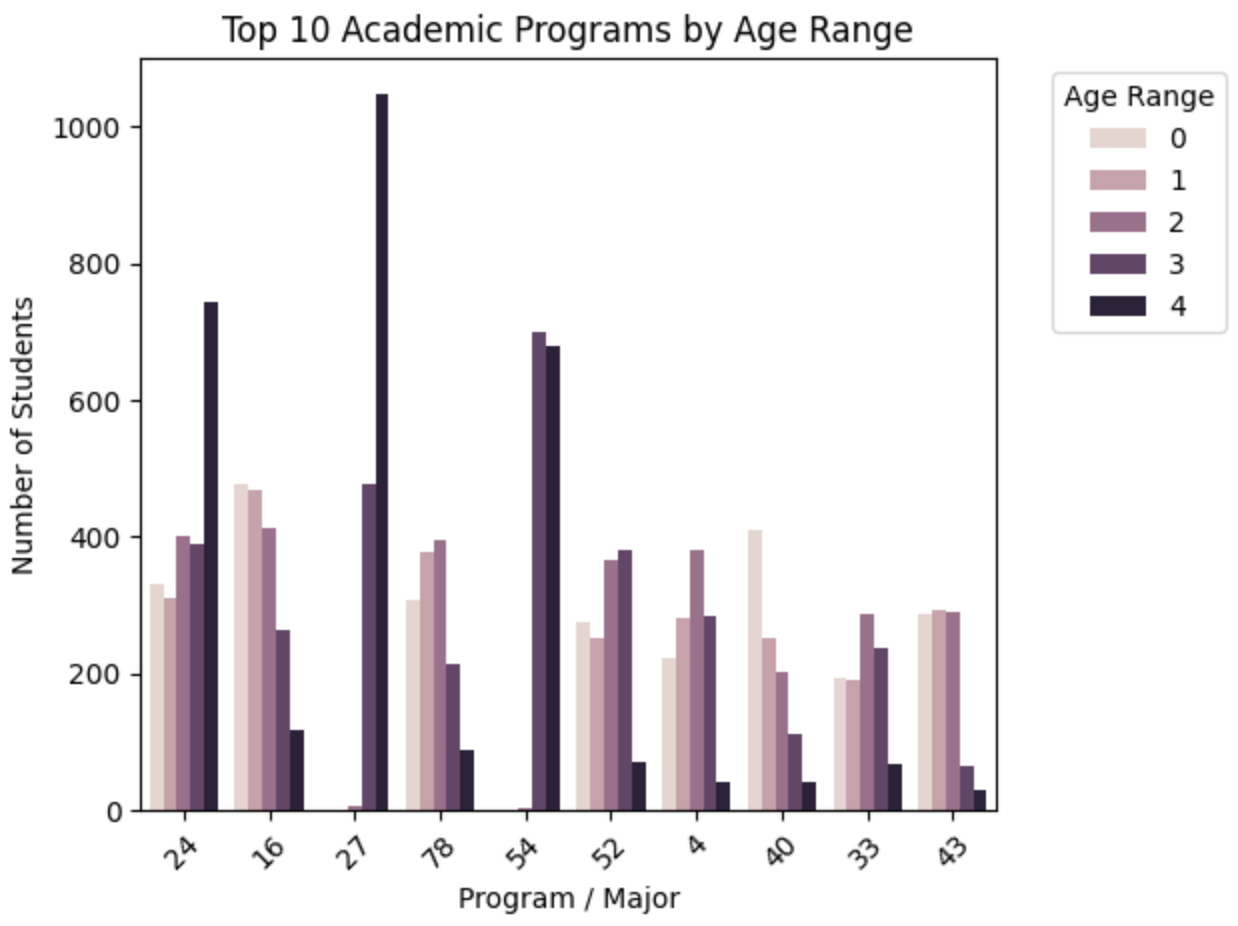
\includegraphics[width=0.7\linewidth]{top_programs_age_range.png}
    \caption{Top Programs vs Age Range}
\end{figure}

\subsection{Study Mode}

\begin{itemize}
    \item Note:\\
    0 : Presencial\\
    1 : Virtual\\
    2 : Remote
    
    \item Program 24\\
    - Most popular program with presencial students.\\
    - Least popular with virtual students.

    \item Program 27, 54\\
    - Least popular program with presencial students.\\
    - Most popular with remote students.

    \item Program 78, 52, 40, 33\\
    - Fairly popular with presencial students.\\
    - Not at all popular with virtual students.

    \item \textbf{Overall}\\
    - Presencial is the most popular study mode and Virtual is the least popular study mode.\\
    - Programs which are popular with presencial have very low participation from virtual.\\
    - Program 24 is the most popular program with presencial students.\\
    - Program 54 is the most popular program with virtual students.\\
    - Program 27 is the most popular program with remote students.
\end{itemize}

\begin{figure}[H]
    \centering
    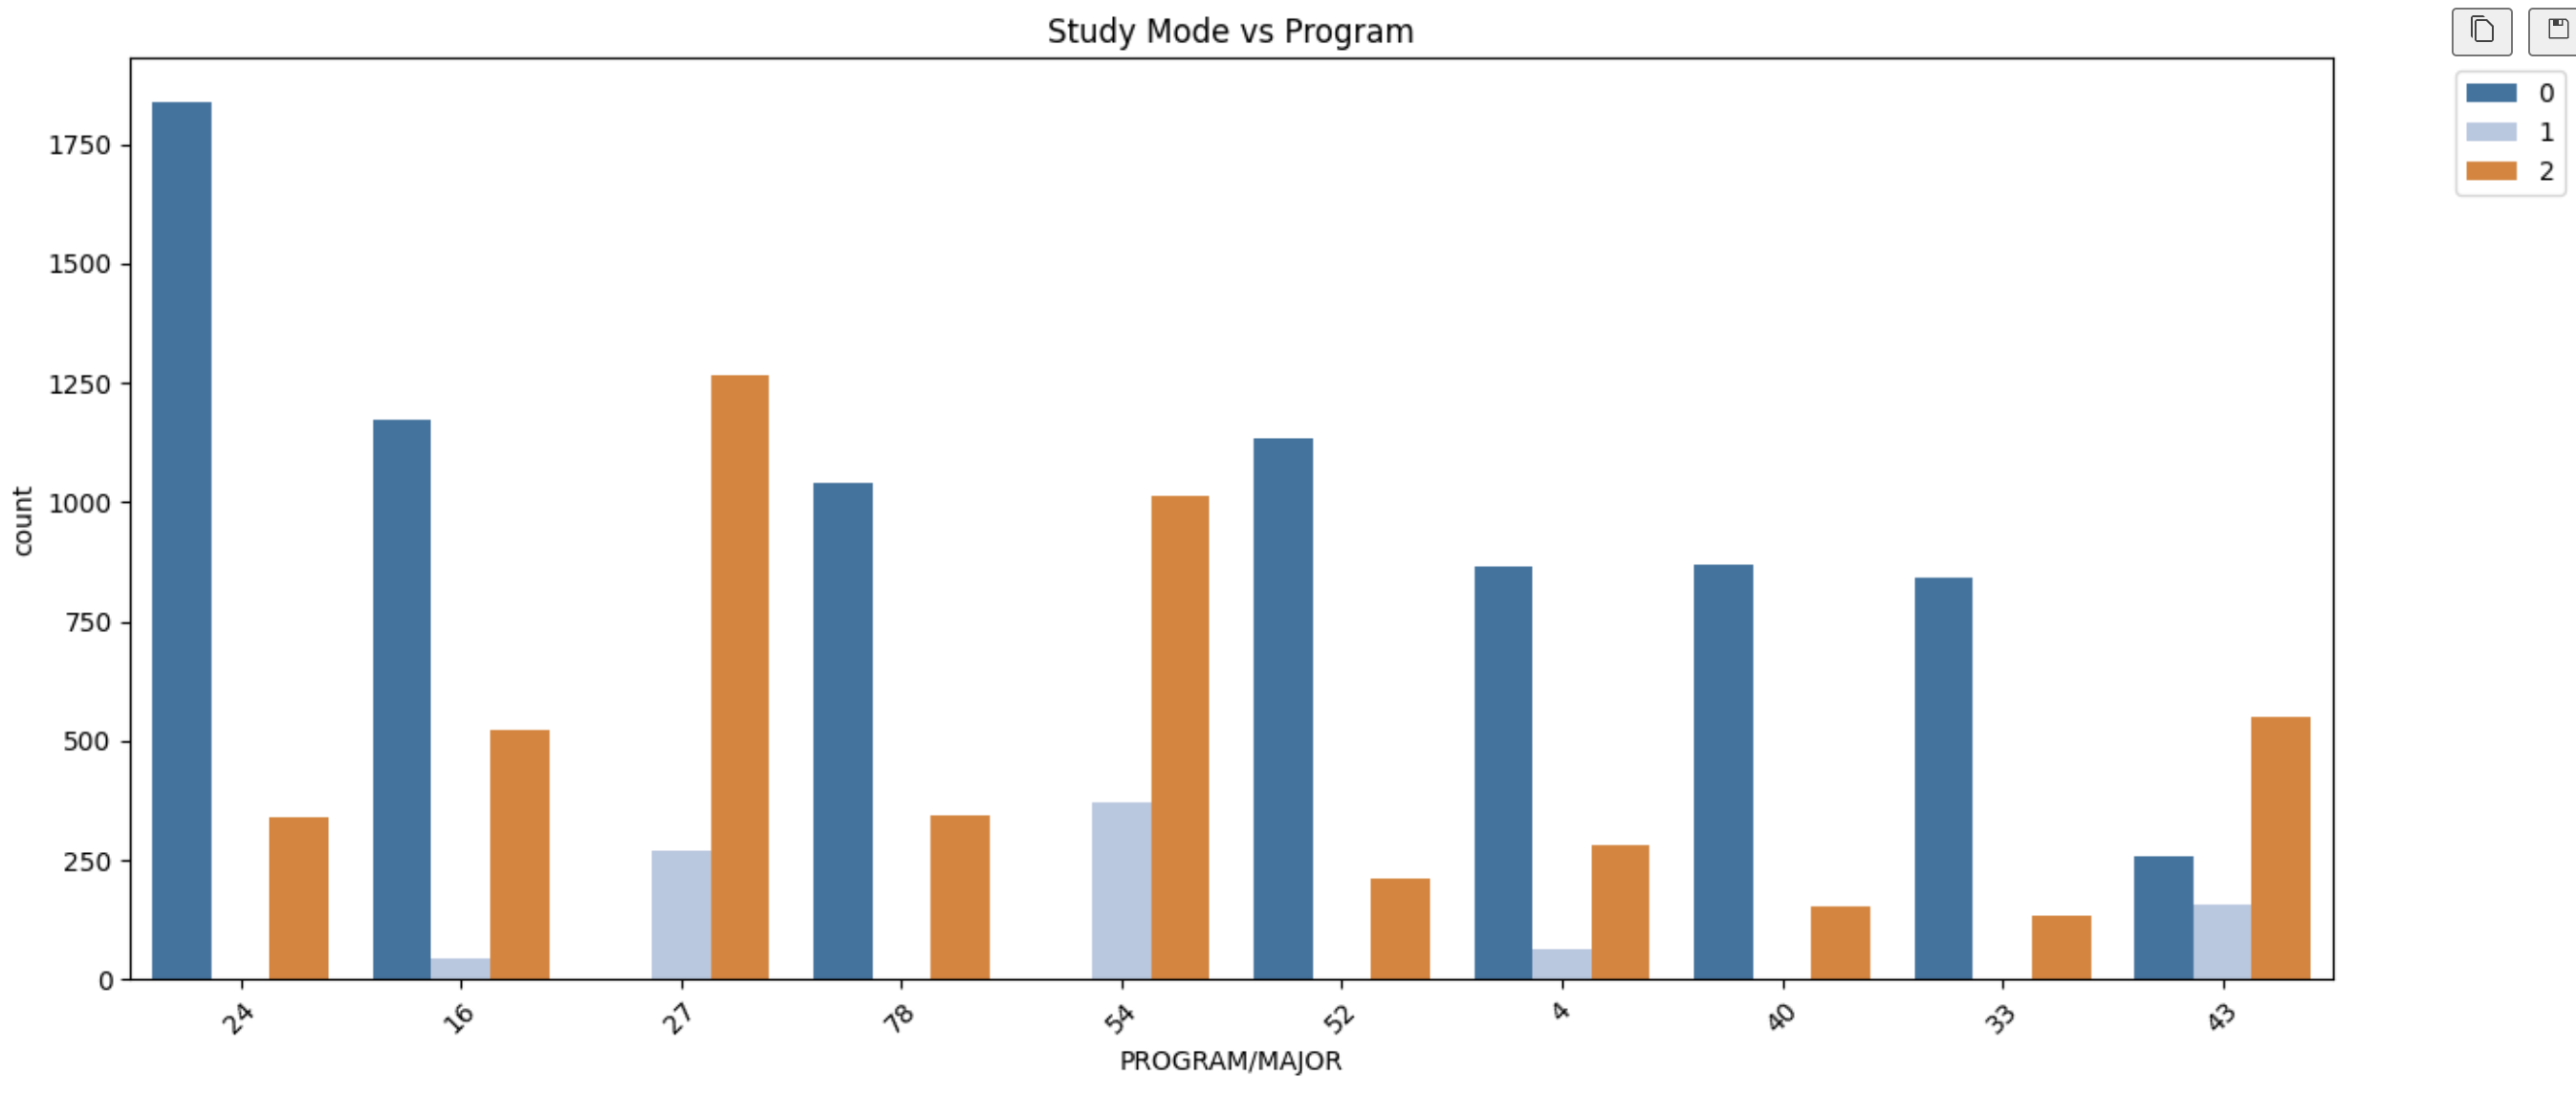
\includegraphics[width=0.9\linewidth]{study_mode.png}
    \caption{Top Programs vs Study Mode}
\end{figure}

\begin{figure}[H]
    \centering
    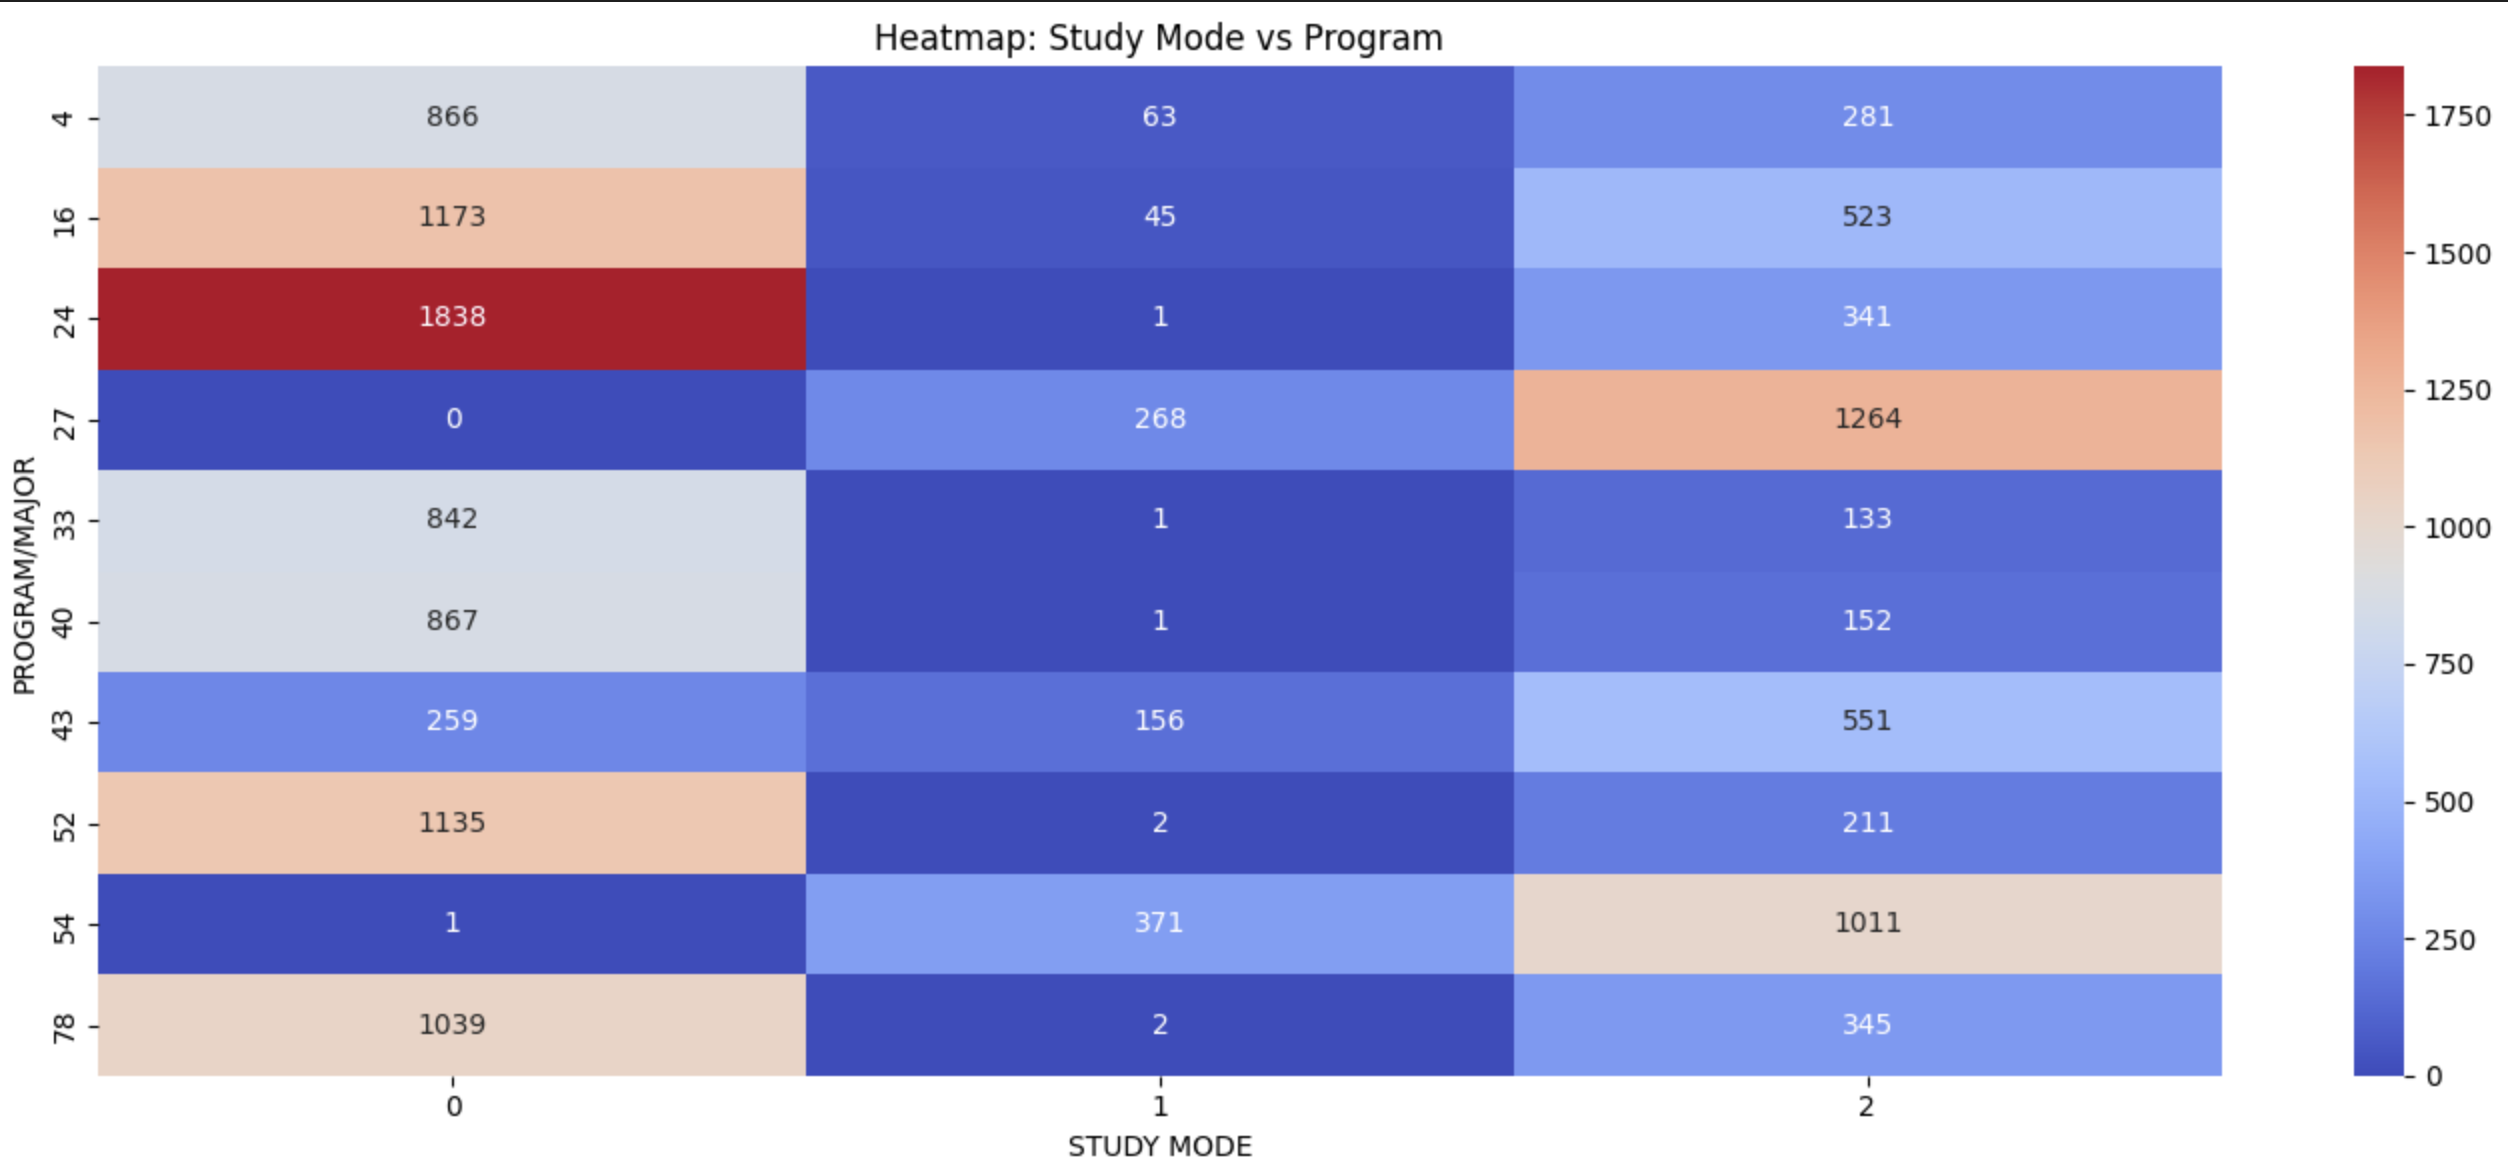
\includegraphics[width=0.9\linewidth]{heatmap_study_mode.png}
    \caption{Heatmap: Top Programs vs Study Mode}
\end{figure}

\section{Tuition Payment Behavior}

\begin{itemize}
    \item Negative trend in tuition payment behavior from 2022 to 2023.
    \item Indicates that the institution's efforts to improve financial literacy or support may not have been effective.
    \item The increase in the percentage of students not paying their tuition could be due to various factors, including economic conditions, changes in student demographics, or institutional policies.
\end{itemize}

\begin{figure}[H]
    \centering
    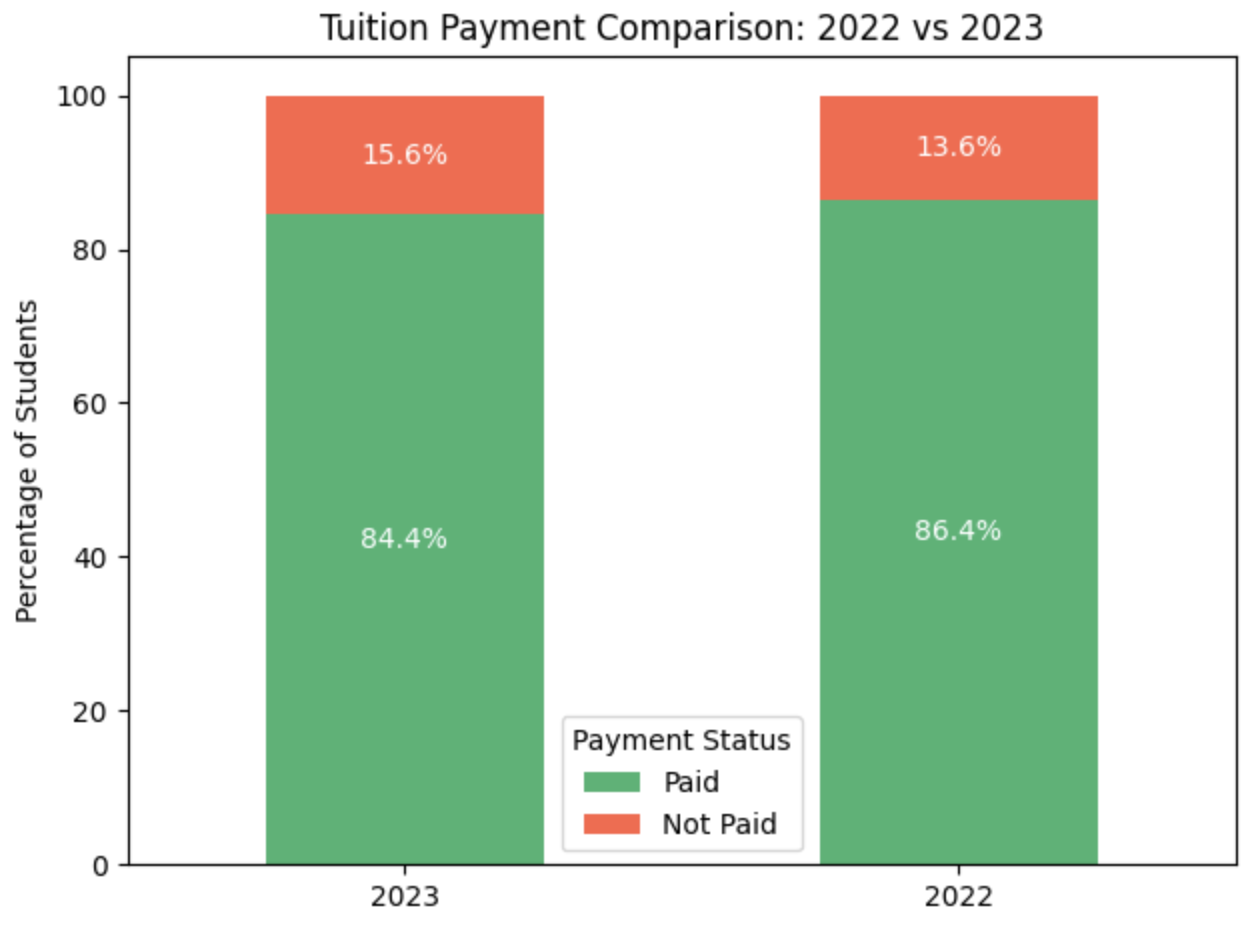
\includegraphics[width=0.7\linewidth]{tuition_payment.png}
    \caption{Tuition Payment: 2022 vs 2023}
\end{figure}

\begin{itemize}
    \item The majority of students maintained their payment status, suggesting a stable financial situation for most students.
    \item A small number of students stopped paying their tuition fees, indicating a potential concern for retention and financial stability.
\end{itemize}

\begin{figure}[H]
    \centering
    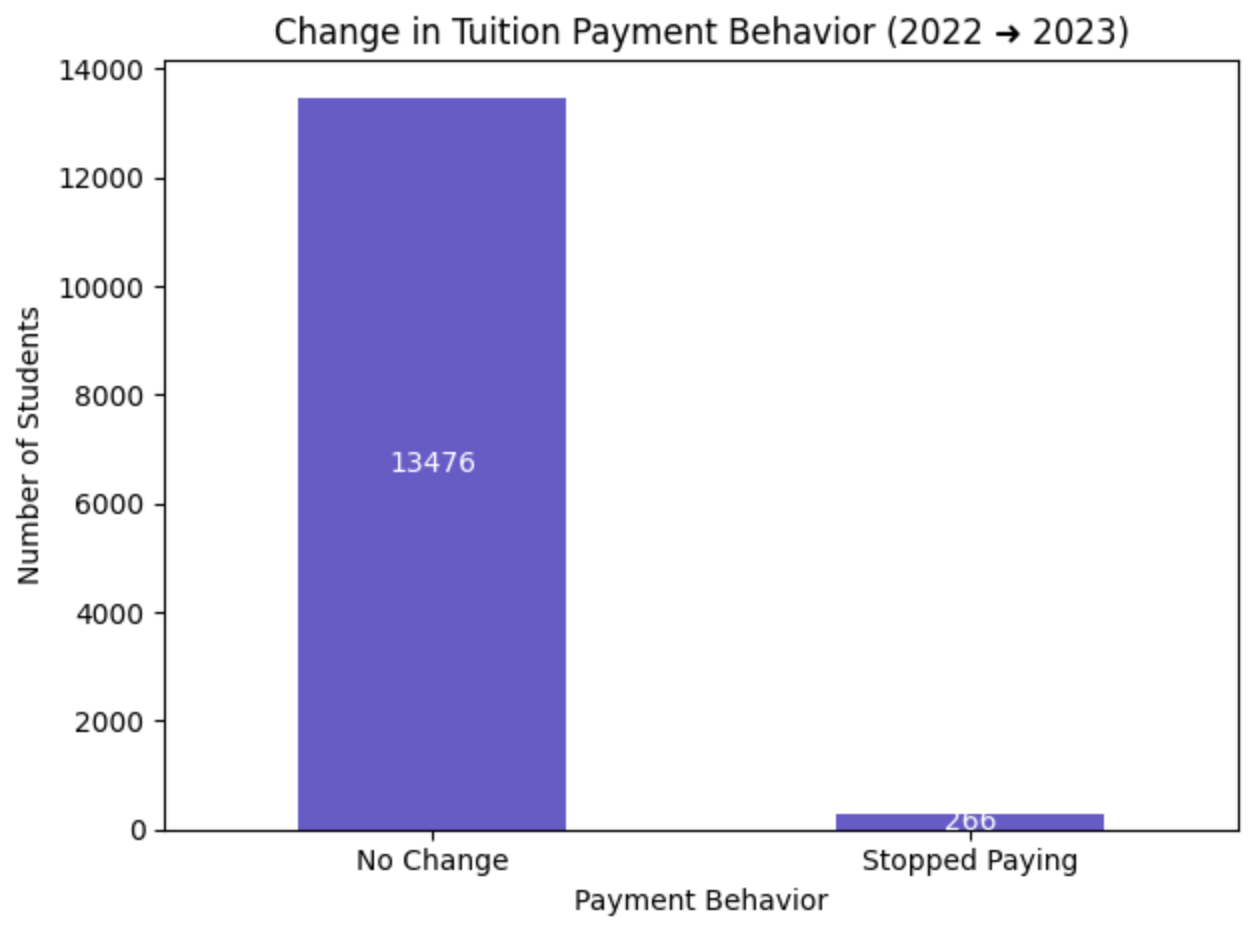
\includegraphics[width=0.7\linewidth]{change_in_tuition_payment.png}
    \caption{Tuition Payment Behavior}
\end{figure}

\begin{itemize}
    \item Female students have a slightly higher percentage of tuition payment compared to male students.
    \item The difference in payment behavior between genders is minimal, indicating similar financial commitment across genders.
    \item Program 24 has the highest percentage of students who paid their tuition fees, indicating strong financial commitment.
    \item Programs 4 and 43 have the lowest percentage of students who paid, suggesting potential financial challenges or disengagement.
    \item The overall trend indicates that most programs have a higher percentage of students who paid their tuition fees compared to those who did not.
\end{itemize}

\begin{figure}[H]
    \centering
    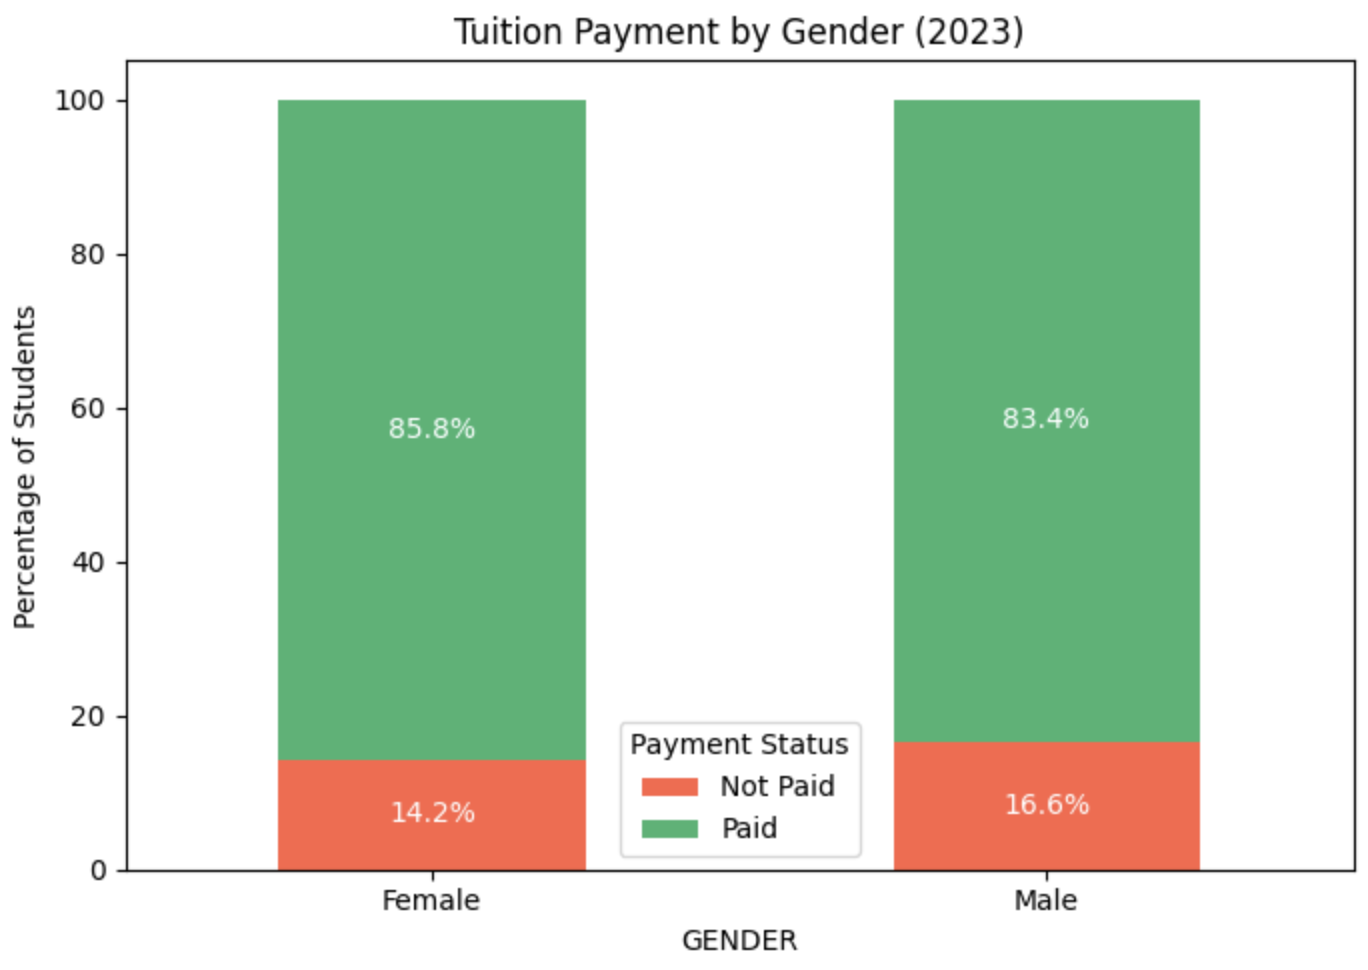
\includegraphics[width=0.55\linewidth]{tuition_payment_gender.png}
    \caption{Tuition Payment vs Gender}
\end{figure}

\begin{figure}[H]
    \centering
    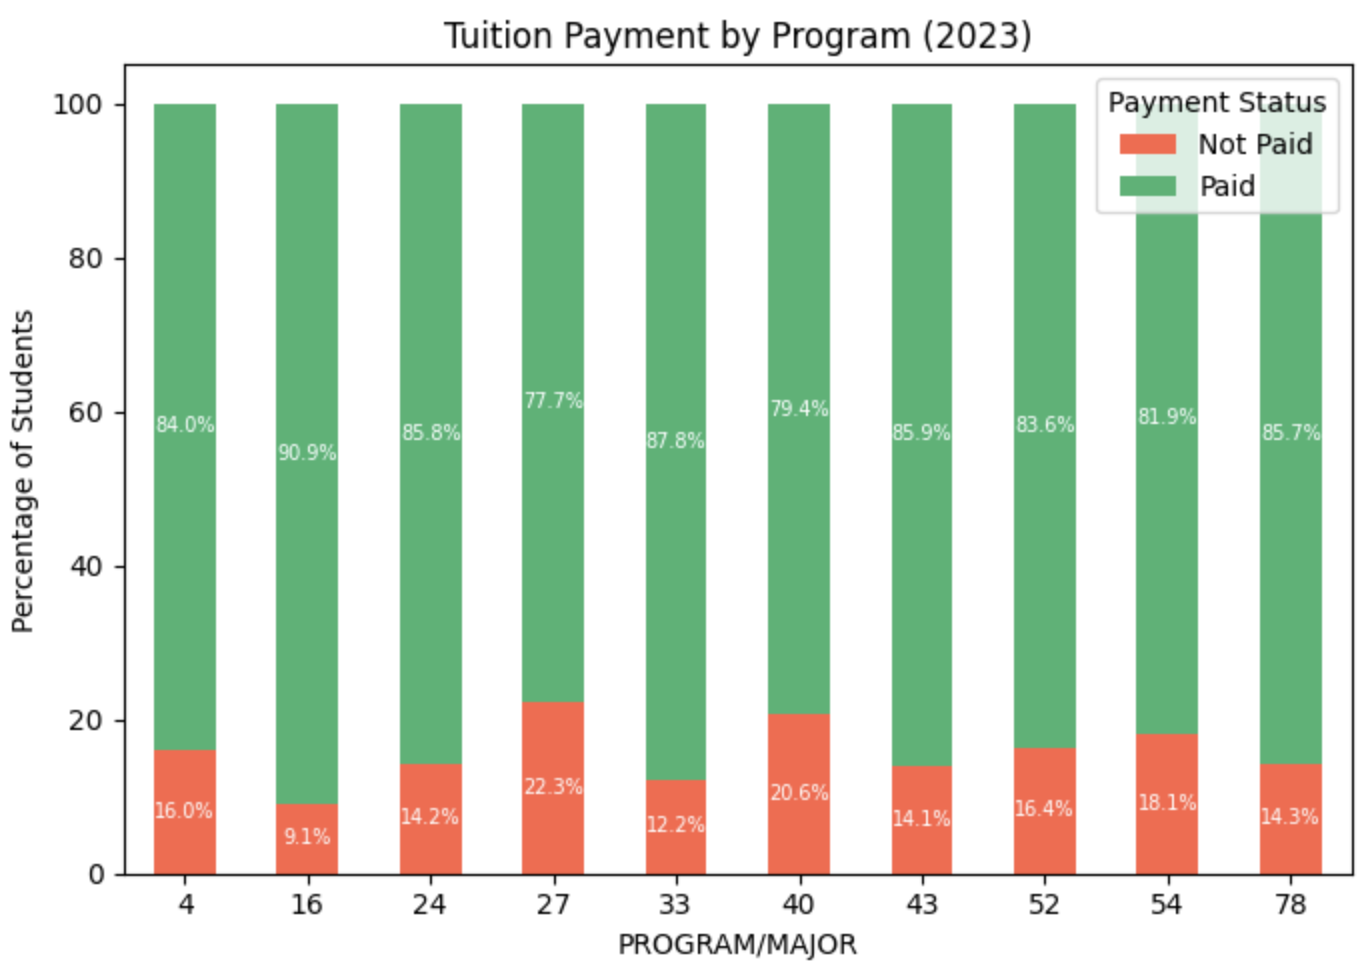
\includegraphics[width=0.55\linewidth]{tuition_payment_program.png}
    \caption{Tuition Payment vs Program}
\end{figure}

\section{Popular Programs and Demographics}

\subsection{Shift/Schedule vs Program}

\begin{itemize}
    \item Note:\\
    0 : Mixto\\
    1 : Noche\\
    2 : Manana\\
    3 : Tarde
    
    \item Program 24\\
    - Popular across all shifts/schedules.\\
    - Most popular program in the "Mixto" shift.

    \item Program 27, 54\\
    - Most popular programs in the "Noche" shifts.

    \item Program 78, 4\\
    - Almost equally popular in "Mixto", "Noche" and "Manana" shifts.

    \item \textbf{Overall}\\
    - "Noche" shift has the highest enrollment across most programs.\\
    - "Tarde" shift has the least enrollment in general by a huge margin.
\end{itemize}

\begin{figure}[H]
    \centering
    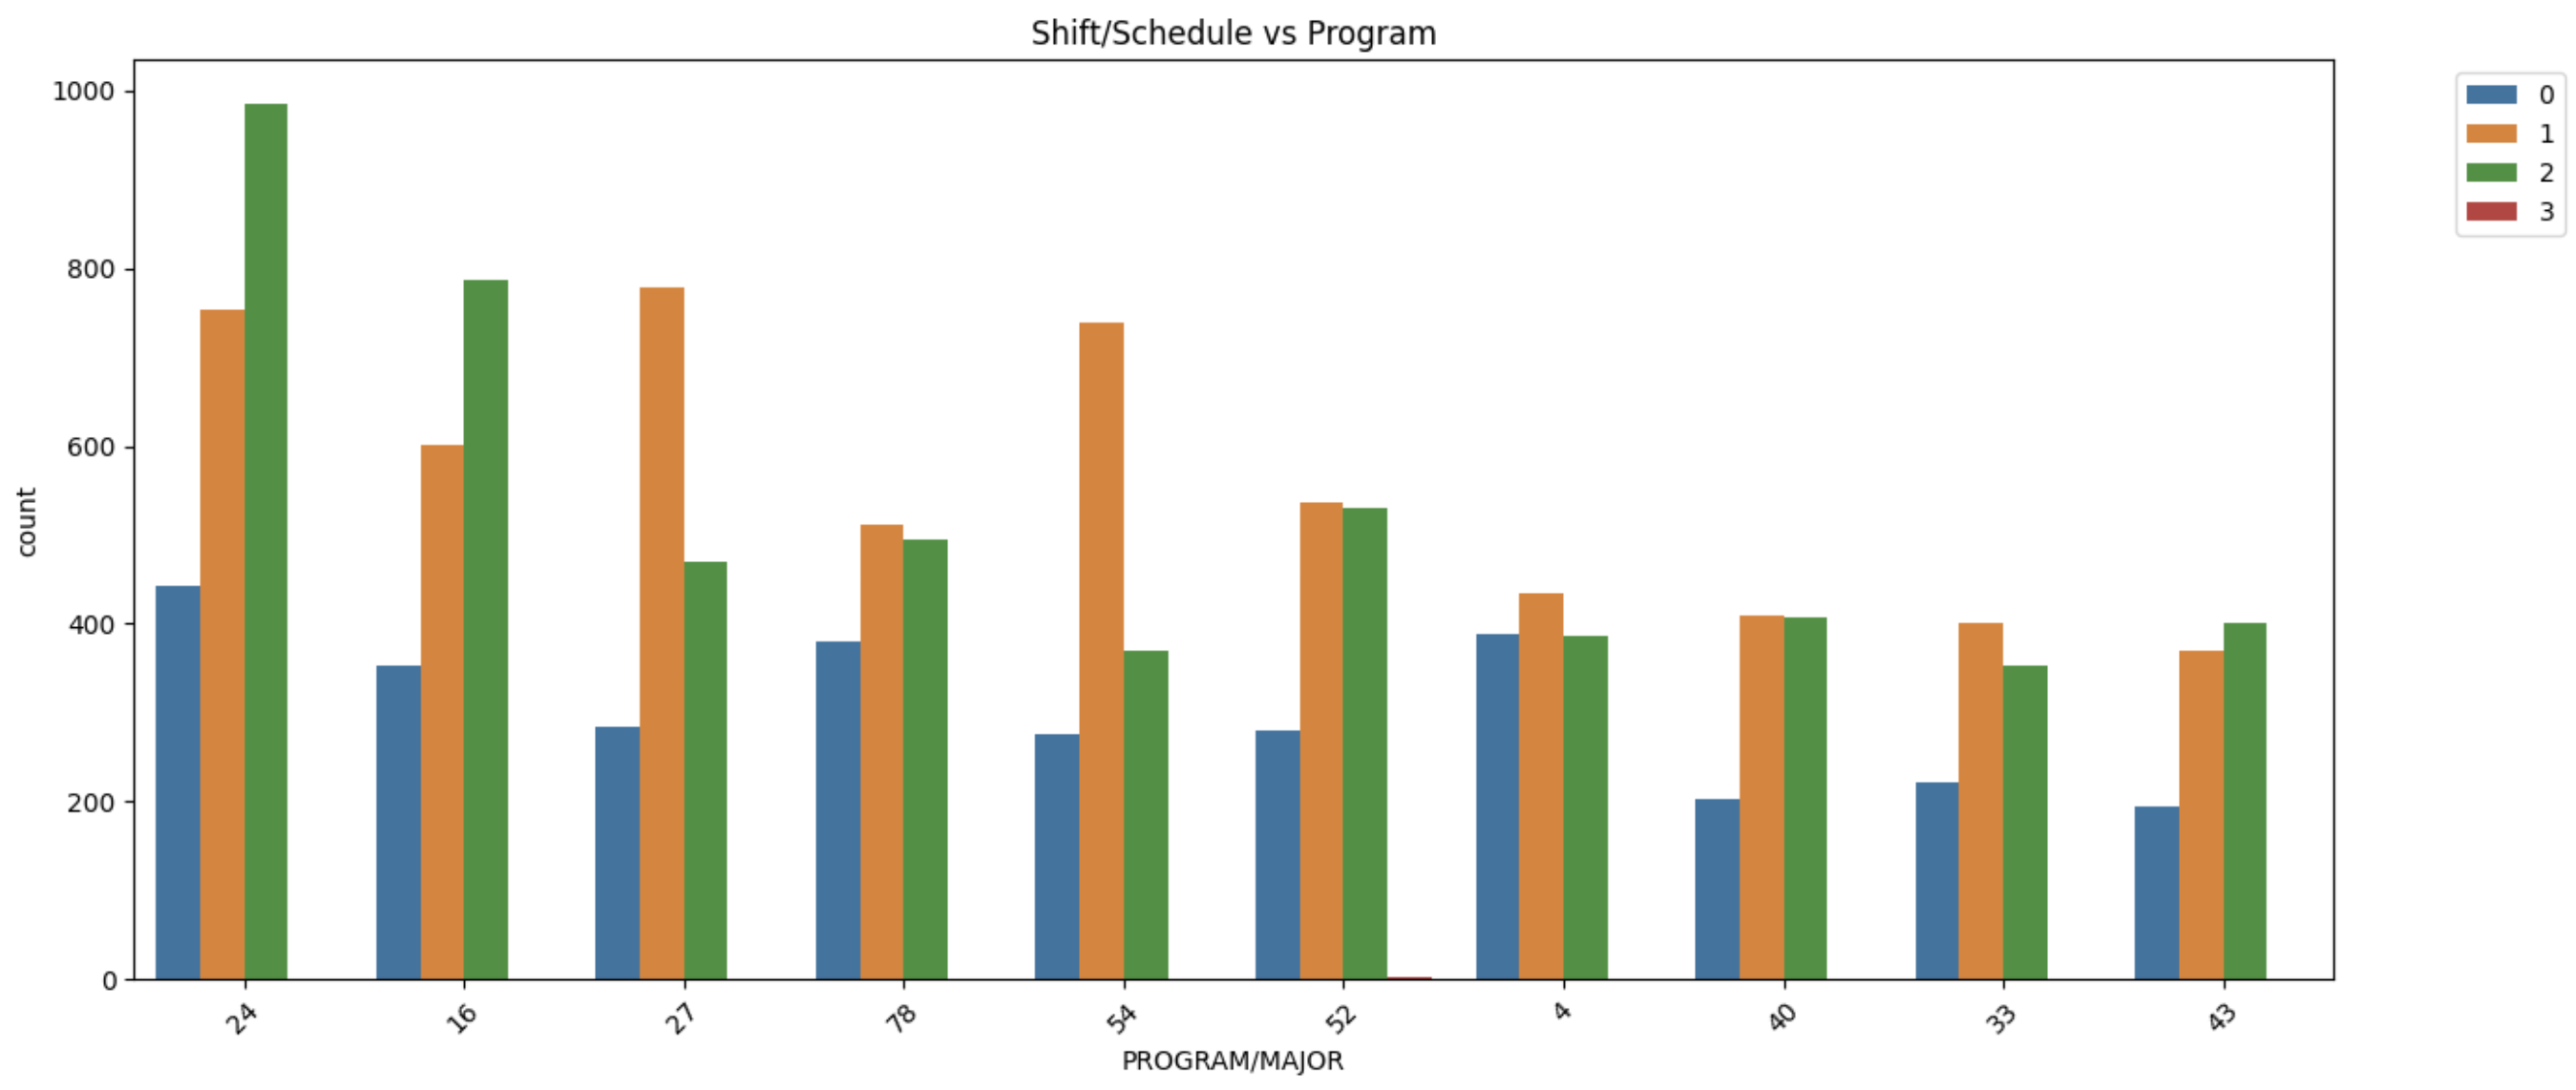
\includegraphics[width=1\linewidth]{shift:schedule.png}
    \caption{Shift/Schedule vs Program}
\end{figure}

\subsection{Benefit Discounts vs Program}

\begin{itemize}
    \item Program 24\\
    - The most popular program across all benefit discount categories.\\
    - Indicates that this program is accessible and attracts students with varying levels of financial support.

    \item Program 27, 54\\
    - Show significant participation from students availing benefit discounts.\\
    - Suggests these programs are particularly appealing to students seeking financial aid.

    \item Program 78, 52\\
    - Moderate participation from students with benefit discounts.\\
    - Indicates a balanced mix of students with and without financial support.

    \item Program 40, 33\\
    - Lower participation from students with benefit discounts compared to other programs.\\
    - May indicate these programs are less reliant on financial aid for enrollment.

    \item \textbf{Overall}\\
    - Programs with higher participation from students availing benefit discounts are likely more affordable or offer better financial aid options.\\
    - Programs like 24 and 27 demonstrate inclusivity and accessibility for students from diverse financial backgrounds.
\end{itemize}

\begin{figure}[H]
    \centering
    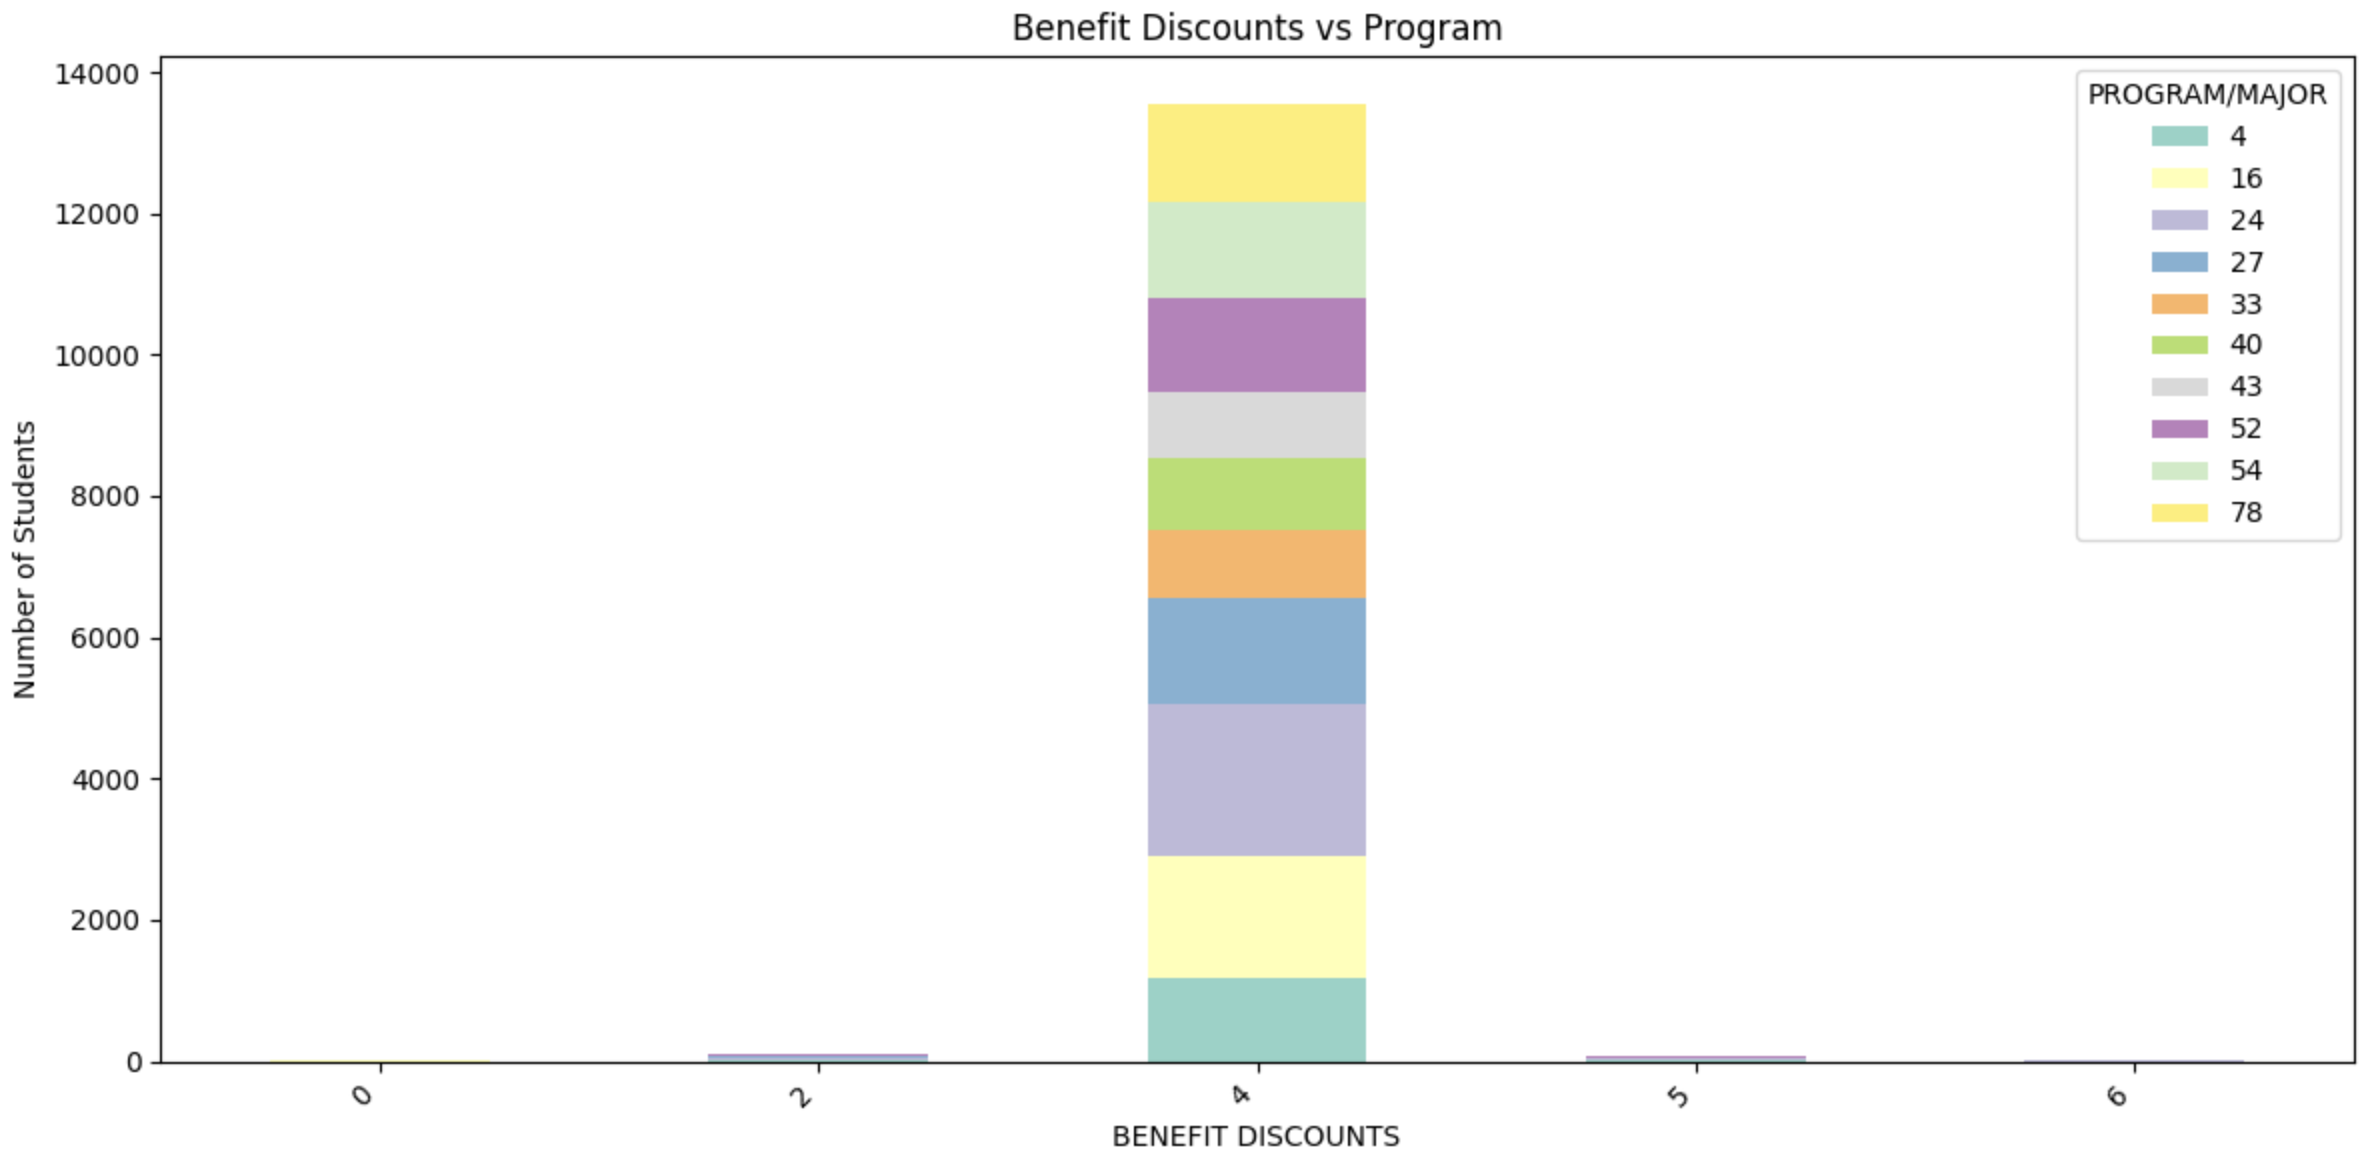
\includegraphics[width=1\linewidth]{benefit_discounts.png}
    \caption{Benefit Discounts vs Program}
\end{figure}

\subsection{Department vs Program}

\begin{itemize}
    \item Program 24\\
    - Strong representation across multiple departments.\\
    - Indicates that this program is widely offered and popular across various departments.

    \item Program 43, 40, 33\\
    - Limited representation in fewer departments.\\
    - Suggests these programs are niche and offered in select departments.
    
    \item \textbf{Overall}\\
    - Department 14 has the highest number of programs.\\
    - Department 16 has the lowest number of programs.\\
    - The distribution of programs across departments reflects the diversity and specialization of academic offerings.
\end{itemize}

\begin{figure}[H]
    \centering
    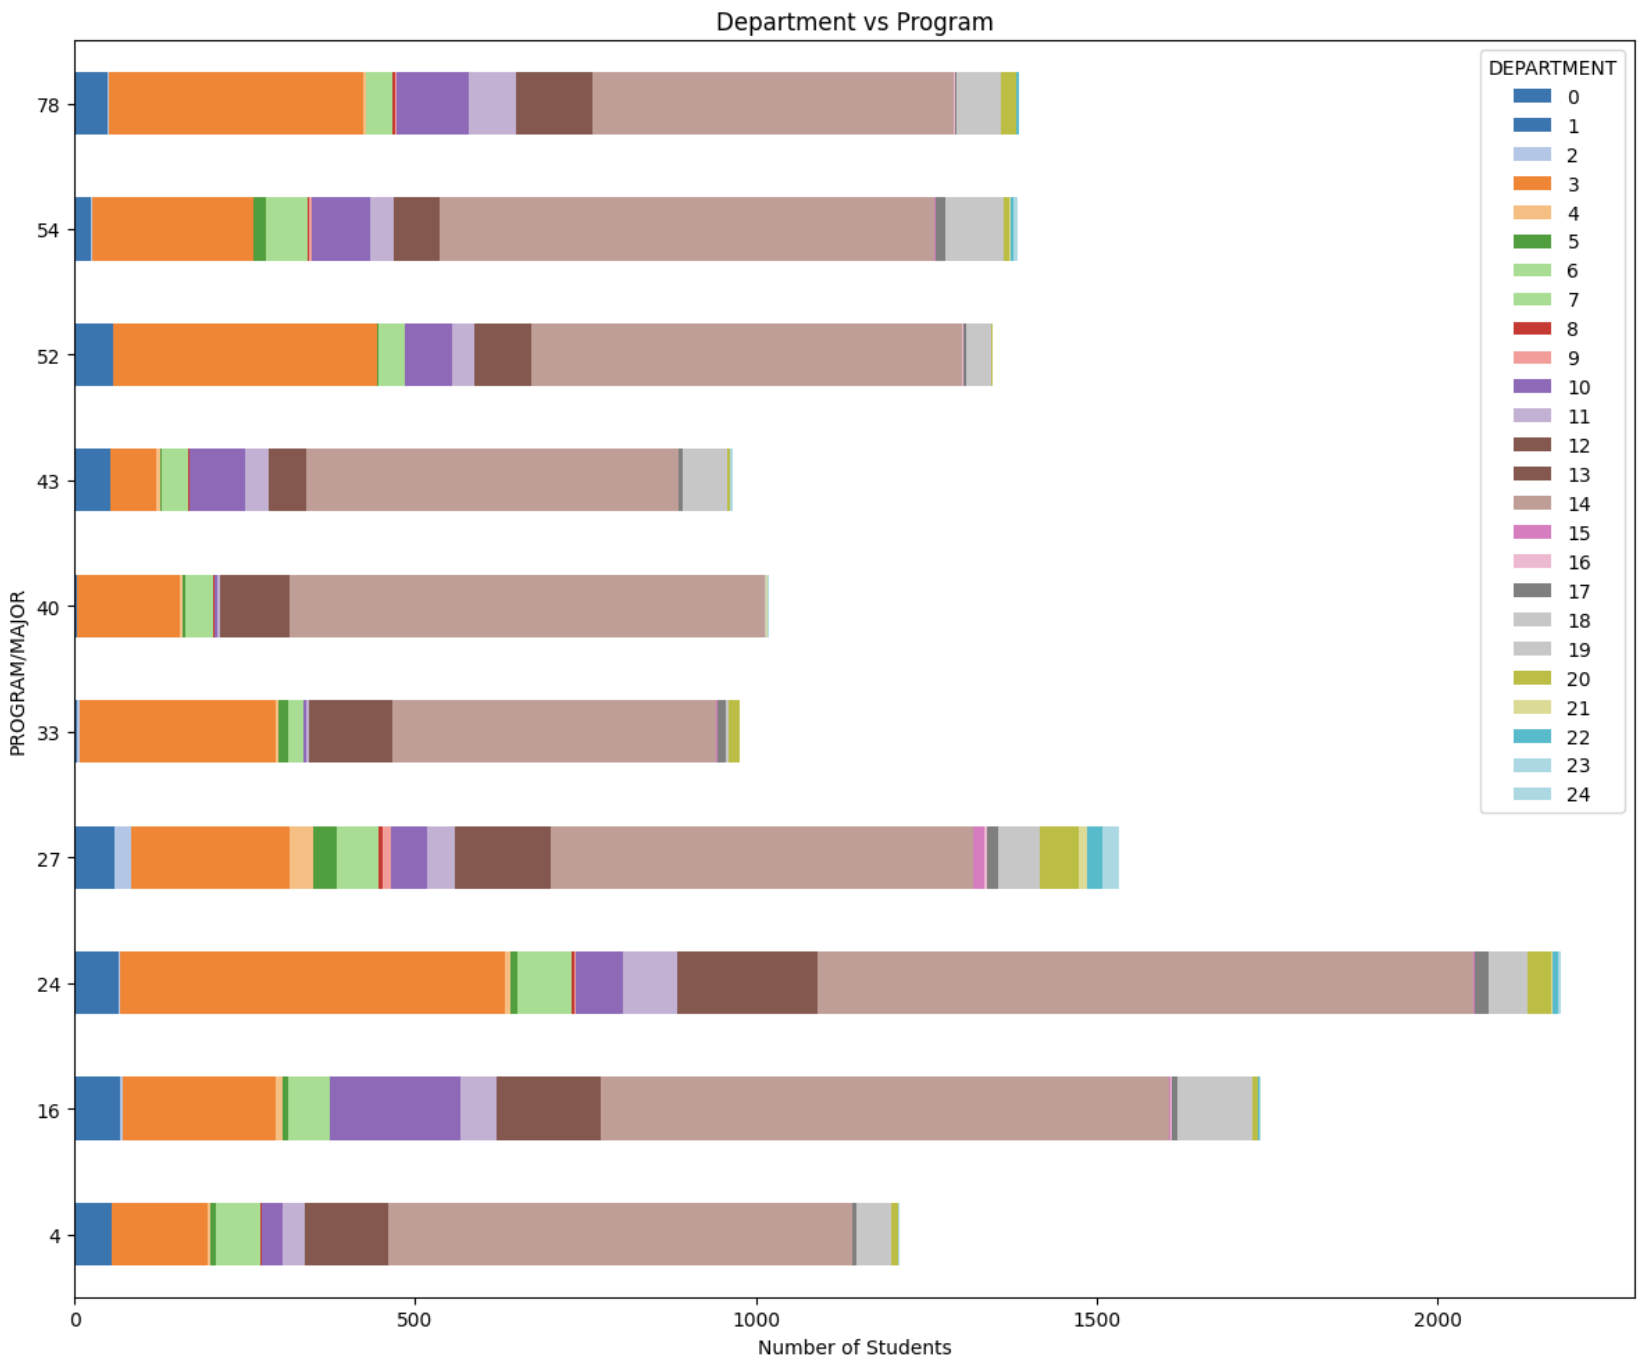
\includegraphics[width=1\linewidth]{department_vs_program.png}
    \caption{Department vs Program}
\end{figure}

\subsection{Enrollment vs Program}

\begin{itemize}
    \item Program 24\\
    - The most popular program across all enrollment types.\\
    - Indicates that this program is widely accessible and attracts a diverse range of students.

    \item Program 43\\
    - Least popular program across all enrollment types.\\
    - Suggests that this program may have specific admission criteria or limited appeal.
    
    \item \textbf{Overall}\\
    - The "Reinstated" enrollment type has the highest number of students across most programs.\\
    - The "New" enrollment type has the lowest number of students across all programs.\\
    - The distribution reflects the diversity of academic offerings and student preferences.
\end{itemize}

\begin{figure}[H]
    \centering
    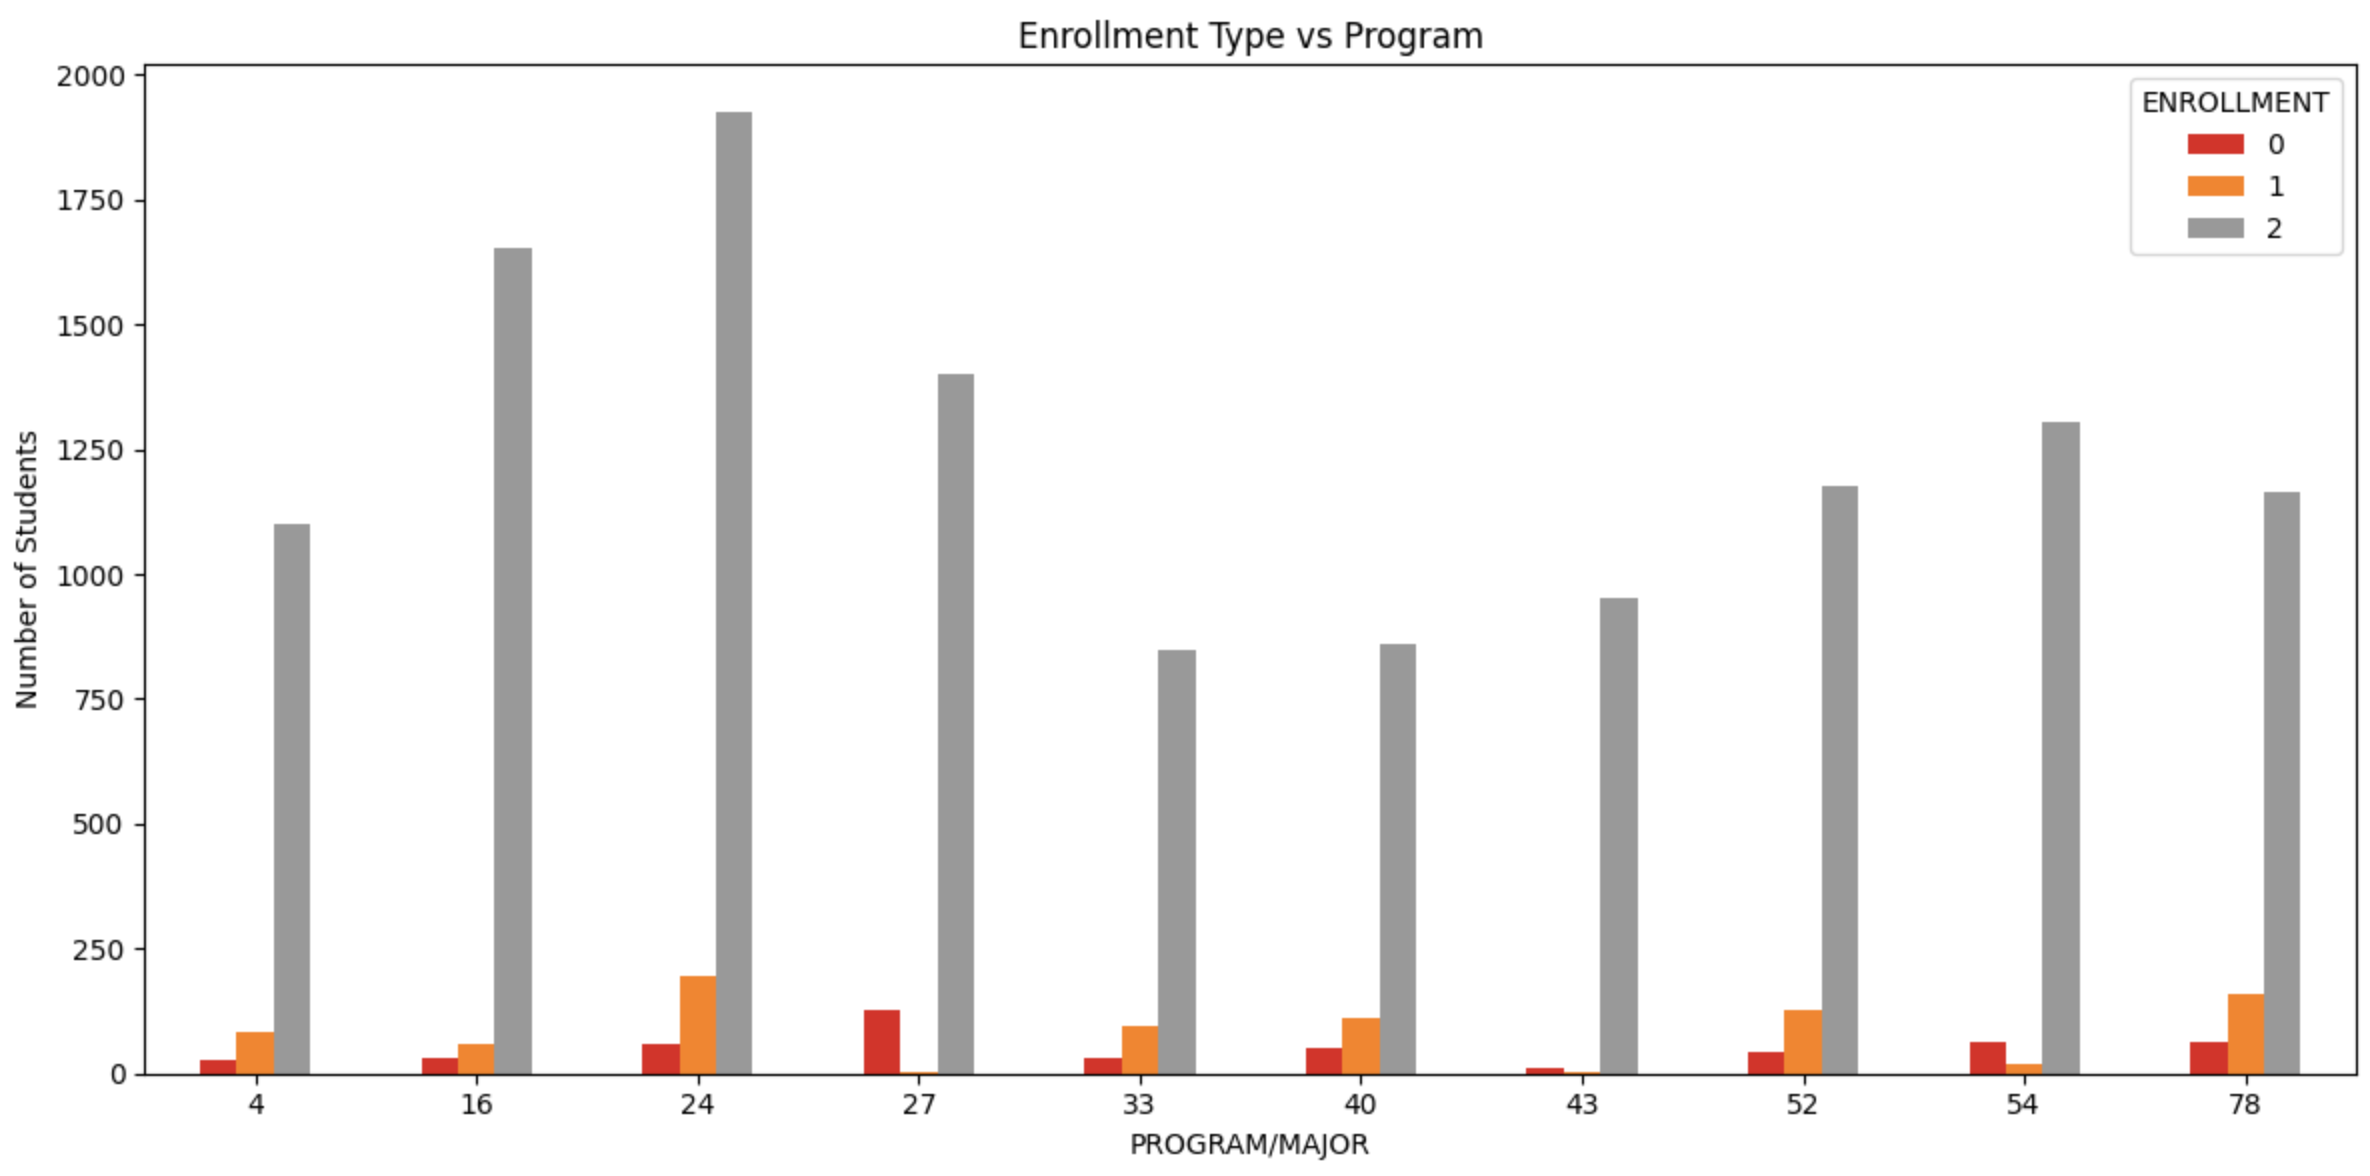
\includegraphics[width=1\linewidth]{enrollment.png}
    \caption{Enrollment vs Program}
\end{figure}

\section{Academic Risk Analysis}

\subsection{Enrolled Courses vs Academic Risk}

\begin{itemize}
    \item Academic risk level 0 (not at risk)\\
    - Wide variation in the number of enrolled courses (ranging from 0 to 6).\\
    - Median is around 2 courses.\\
    - Indicates high diversity in course load among students not at risk.

    \item Academic risk levels 1 to 5\\
    - As risk increases, the number of enrolled courses becomes more consistent and increases linearly (1 to 5 courses).\\
    - No variation at each risk level — students with higher risk seem to be taking exactly as many courses as their risk level.\\
    - Suggests a potential direct mapping between number of courses and risk level from 1 to 5 (e.g., 3 enrolled courses → 3 at-risk courses).

    \item \textbf{Overall}\\ \\
    \ding{212} The violin plot gives similar information as the box plot but also shows the density/distribution of enrolled courses:\\
    - For risk level 0, there are multiple peaks at 1, 2, and 3 courses.\\
    - Suggests several common course loads among students not at risk.\\
    - For risk levels 1–5, the density collapses into a single point at each risk level (e.g., risk level 3 = 3 enrolled courses).\\ \\
    \ding{212} Again, implies no variation in course loads for higher-risk students, which might be due to:\\
    - Data preprocessing (e.g., risk level might be equal to number of courses).\\
    - An actual policy (e.g., assigning risk based on the number of courses).
\end{itemize}

\begin{figure}[H]
    \centering
    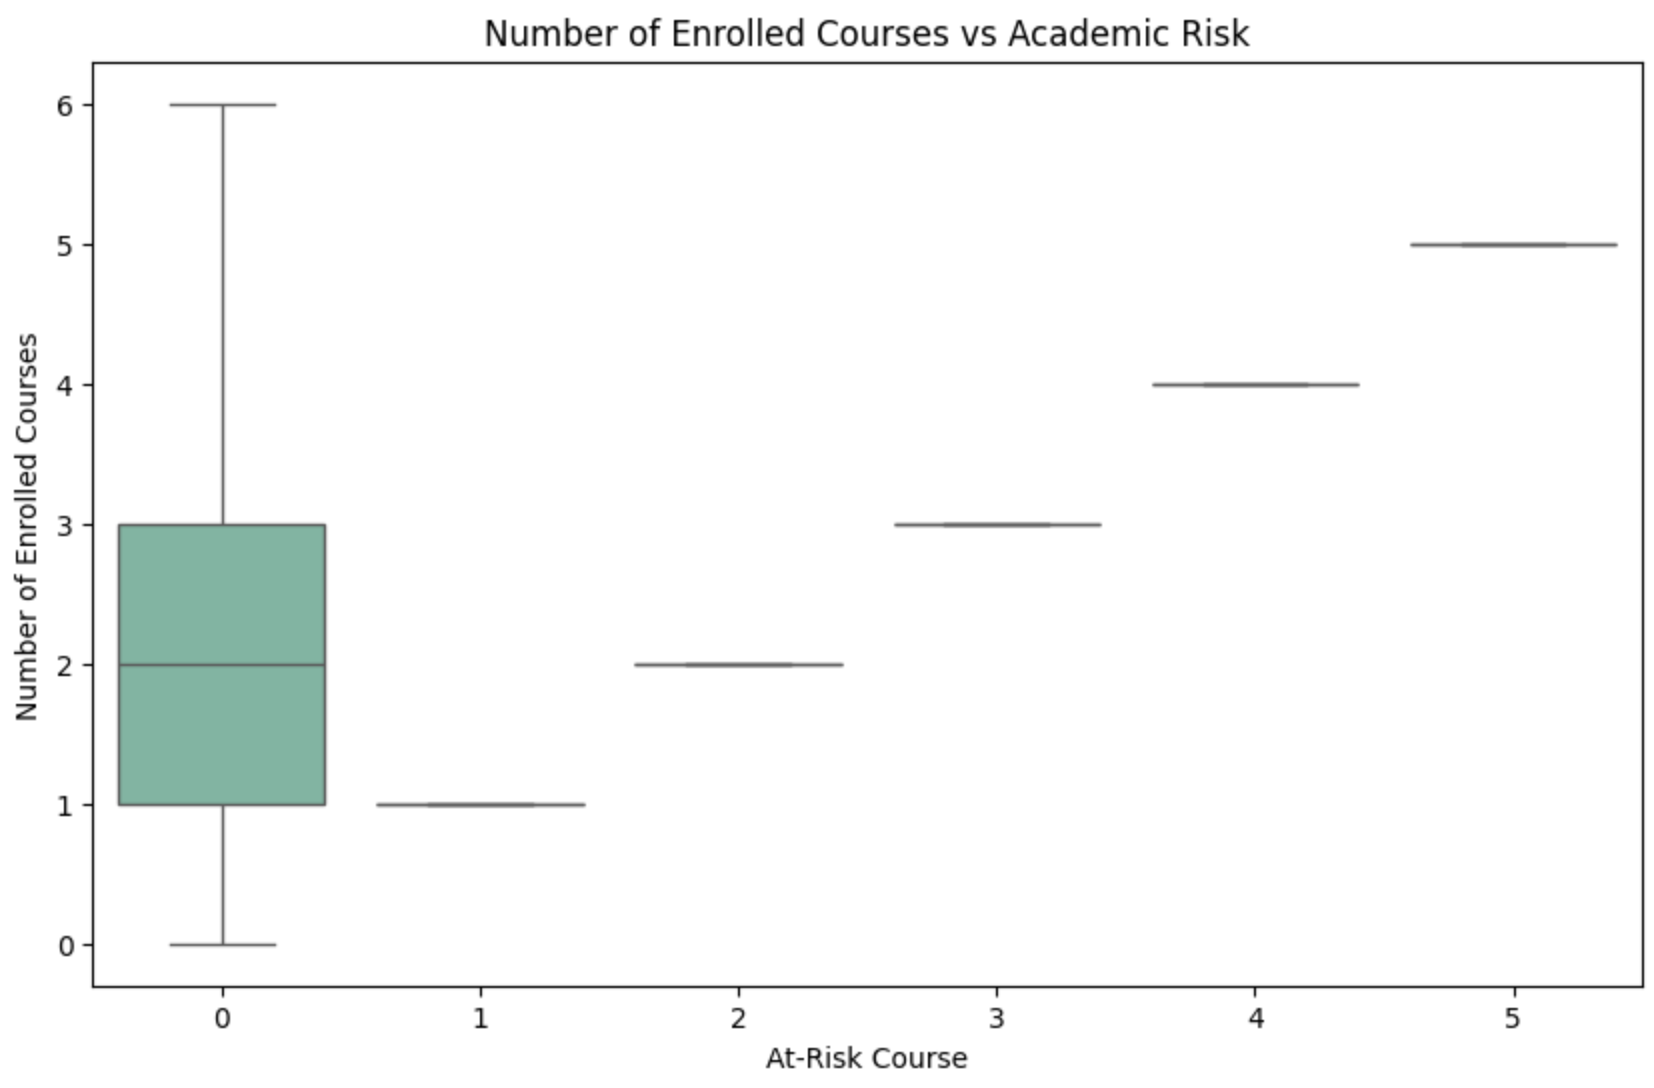
\includegraphics[width=1\linewidth]{boxplot_academic_risk.png}
    \caption{Number of Enrolled Courses vs Academic Risk}
\end{figure}

\begin{figure}[H]
    \centering
    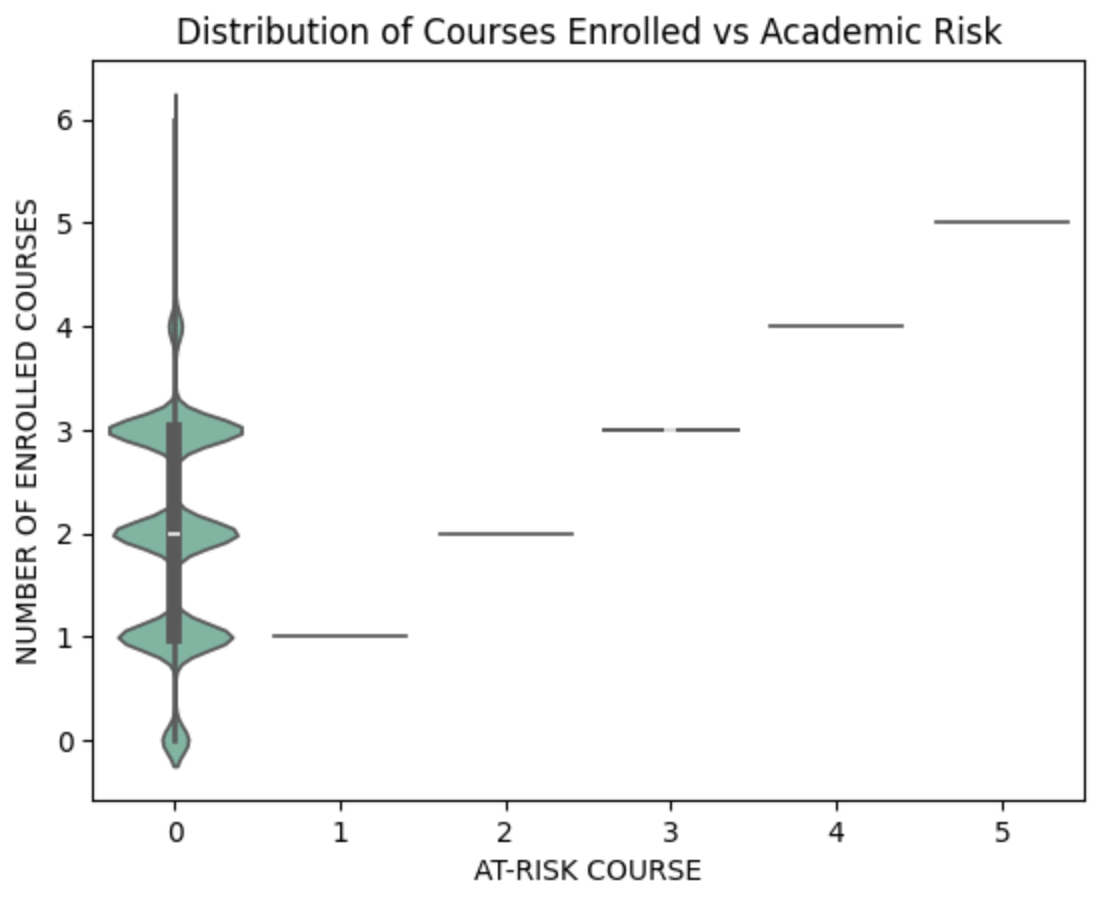
\includegraphics[width=0.8\linewidth]{violinplot_academic_risk.png}
    \caption{Distribution of Enrolled Courses vs Academic Risk}
\end{figure}

\section{Conclusion}
We explored and analyzed student enrollment data from a Peruvian university, highlighting the key trends. The findings show that enrollment patterns are influenced by gender, study mode, age range, while academic risk is closely associated with course load. Overall, this analysis demonstrates the value of data-driven insights in supporting institutional decisions, improving student outcomes, and optimizing academic resource allocation.

\end{document}
